\documentclass[8pt,aspectratio=169]{beamer}
\usetheme{Madrid}
\usepackage{graphicx}
\usepackage{booktabs}
\usepackage{adjustbox}
\usepackage{multicol}
\usepackage{amsmath}
\usepackage{amssymb}
\usepackage{tikz}
\usepackage{hyperref}
\usepackage{algorithm}
\usepackage{algorithmic}
\usepackage{colortbl}
\usepackage{pgfplots}
\pgfplotsset{compat=1.18}

% TikZ libraries for comics, diagrams, stakeholder maps
\usetikzlibrary{arrows.meta,positioning,shapes.callouts,shapes.geometric,decorations.pathreplacing}

% Color definitions
\definecolor{mlblue}{RGB}{0,102,204}
\definecolor{mlpurple}{RGB}{51,51,178}
\definecolor{mllavender}{RGB}{173,173,224}
\definecolor{mllavender2}{RGB}{193,193,232}
\definecolor{mllavender3}{RGB}{204,204,235}
\definecolor{mllavender4}{RGB}{214,214,239}
\definecolor{mlorange}{RGB}{255, 127, 14}
\definecolor{mlgreen}{RGB}{44, 160, 44}
\definecolor{mlred}{RGB}{214, 39, 40}
\definecolor{mlgray}{RGB}{127, 127, 127}
\definecolor{lightgray}{RGB}{240, 240, 240}
\definecolor{midgray}{RGB}{180, 180, 180}

% NEW COLORS for mini-lecture
\definecolor{dfteal}{RGB}{0,128,128}
\definecolor{dfred}{RGB}{180,30,30}

% Backward compatibility
\colorlet{MLPurple}{mlpurple}
\colorlet{MLBlue}{mlblue}
\colorlet{MLOrange}{mlorange}
\colorlet{MLGreen}{mlgreen}
\colorlet{MLRed}{mlred}
\colorlet{MLLavender}{mllavender}
\colorlet{MLGray}{mlgray}

% Theme colors (exact Madrid settings)
\setbeamercolor{palette primary}{bg=mllavender3,fg=mlpurple}
\setbeamercolor{palette secondary}{bg=mllavender2,fg=mlpurple}
\setbeamercolor{palette tertiary}{bg=mllavender,fg=white}
\setbeamercolor{palette quaternary}{bg=mlpurple,fg=white}
\setbeamercolor{structure}{fg=mlpurple}
\setbeamercolor{section in toc}{fg=mlpurple}
\setbeamercolor{subsection in toc}{fg=mlblue}
\setbeamercolor{title}{fg=mlpurple}
\setbeamercolor{frametitle}{fg=mlpurple,bg=mllavender3}
\setbeamercolor{block title}{bg=mllavender2,fg=mlpurple}
\setbeamercolor{block body}{bg=mllavender4,fg=black}
\setbeamertemplate{navigation symbols}{}
\setbeamertemplate{itemize items}[circle]
\setbeamertemplate{enumerate items}[default]
\setbeamersize{text margin left=5mm,text margin right=5mm}

% Footer
\setbeamertemplate{footline}{
  \leavevmode%
  \hbox{%
    \begin{beamercolorbox}[wd=.333333\paperwidth,ht=2.25ex,dp=1ex,center]{author in head/foot}%
      \usebeamerfont{author in head/foot}Methods and Algorithms
    \end{beamercolorbox}%
    \begin{beamercolorbox}[wd=.333333\paperwidth,ht=2.25ex,dp=1ex,center]{title in head/foot}%
      \usebeamerfont{title in head/foot}MSc Data Science
    \end{beamercolorbox}%
    \begin{beamercolorbox}[wd=.333333\paperwidth,ht=2.25ex,dp=1ex,right]{date in head/foot}%
      \usebeamerfont{date in head/foot}\insertframenumber{} / \inserttotalframenumber\hspace*{2ex}
    \end{beamercolorbox}}%
  \vskip0pt%
}

\newcommand{\bottomnote}[1]{%
\vfill
\vspace{-2mm}
\textcolor{mllavender2}{\rule{\textwidth}{0.4pt}}
\vspace{1mm}
\footnotesize
\textbf{#1}
}

\newenvironment{compactlist}{%
  \begin{itemize}%
    \setlength{\itemsep}{2pt}%
    \setlength{\parskip}{0pt}%
    \setlength{\parsep}{0pt}%
}{%
  \end{itemize}%
}

\newcommand{\highlight}[1]{\textcolor{mlorange}{\textbf{#1}}}
\newcommand{\mathbold}[1]{\boldsymbol{#1}}

\title[L02: Logistic Regression Full Lecture]{L02: Logistic Regression}
\subtitle{Full Lecture: Mathematical Foundations, Inference, and Credit Scoring}
\author{Methods and Algorithms}
\institute{MSc Data Science}
\date{}
\begin{document}

%% === SECTION 0: OPENING ===

%% ================================================================
%% FRAME 1: Title Page
%% ================================================================
\begin{frame}
\titlepage
\end{frame}

%% ================================================================
%% FRAME 2: Opening Comic -- XKCD #1132
%% ================================================================
\begin{frame}[t]{The Eternal Debate}
\begin{columns}[T]
\column{0.55\textwidth}
\small
\textbf{Frequentist vs.\ Bayesian}

\begin{compactlist}
\item A neutrino detector signals ``the sun has gone nova''
\item The frequentist: ``the p-value is below 0.05, so we reject the null''
\item The Bayesian: ``given my prior that the sun exists, I bet the detector is lying''
\end{compactlist}

\vspace{2mm}
\scriptsize
Logistic regression lives in this tension: the model gives you a probability, but how you \emph{interpret} it depends on your framework. Today we build the math that both camps agree on.

\column{0.42\textwidth}
\vspace{2mm}
\includegraphics[height=0.55\textheight]{images/1132_frequentist_bayesian.png}
\end{columns}

\bottomnote{XKCD \#1132 by Randall Munroe (CC BY-NC 2.5) -- ``Is the sun going to explode?''}
\end{frame}

%% ================================================================
%% FRAME 3: Learning Objectives
%% ================================================================
\begin{frame}[t]{Learning Objectives}
\begin{columns}[T]
\column{0.55\textwidth}
\small
\textbf{After this lecture you will be able to:}

\begin{enumerate}
\setlength{\itemsep}{3pt}
\item \textbf{Derive} the MLE for logistic regression via the gradient of the log-likelihood (Analyze)
\item \textbf{Evaluate} classification performance using ROC, precision-recall, calibration, and Gini (Evaluate)
\item \textbf{Analyze} model fit via deviance, Wald test, LRT, AIC/BIC, and Hosmer--Lemeshow (Analyze)
\item \textbf{Apply} logistic regression to credit scoring with Basel-compliant PD estimation (Apply)
\item \textbf{Compare} regularization strategies (L1, L2, Elastic Net) and their effect on model selection (Evaluate)
\end{enumerate}

\column{0.42\textwidth}
\footnotesize
\vspace{4mm}
\fcolorbox{mlpurple}{mllavender4}{\parbox{0.88\columnwidth}{%
\textbf{Finance application:}

\vspace{2mm}
Every objective maps to a real credit-scoring task: PD estimation, model validation, regulatory reporting, and scorecard deployment under Basel~II/III.
}}
\end{columns}

\bottomnote{Bloom's taxonomy levels 3--5: Apply, Analyze, Evaluate}
\end{frame}

%% ================================================================
%% FRAME 4: WHY -- Core Tension
%% ================================================================
\begin{frame}[t]{Why Would a Bank Want a Probability Instead of a Score?}
\begin{columns}[T]
\column{0.55\textwidth}
\small
\textbf{The Core Tension}

\begin{compactlist}
\item A linear model predicts $\hat{y} = \mathbf{w}^\top \mathbf{x} + b$, which can be $-3.2$ or $+1.7$
\item But a bank needs $P(\text{default}) \in [0,1]$ for capital reserves
\item Thresholding a raw score at zero gives a decision, not a probability
\end{compactlist}

\vspace{2mm}
\scriptsize
The sigmoid function bridges this gap: it maps any real number to $(0,1)$, turning an unbounded score into a calibrated probability of default.

\begin{block}{Insight}
\scriptsize Classification demands a probability, but a linear model gives you an unbounded number. The sigmoid is the mathematical bridge, and everything else follows from maximum likelihood.
\end{block}

\column{0.42\textwidth}
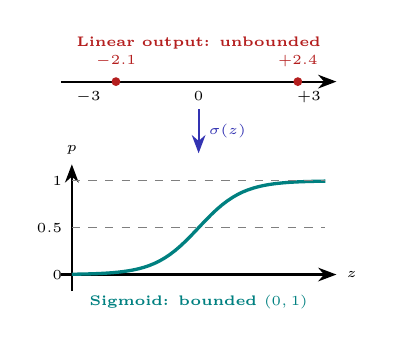
\begin{tikzpicture}[scale=0.7]
% Number line showing linear output
\draw[-{Stealth}, thick] (-0.5,3.5) -- (4.5,3.5);
\node[font=\tiny, below] at (0,3.5) {$-3$};
\node[font=\tiny, below] at (2,3.5) {$0$};
\node[font=\tiny, below] at (4,3.5) {$+3$};
\fill[dfred] (0.5,3.5) circle (0.08);
\fill[dfred] (3.8,3.5) circle (0.08);
\node[font=\tiny, dfred, above] at (0.5,3.6) {$-2.1$};
\node[font=\tiny, dfred, above] at (3.8,3.6) {$+2.4$};
\node[font=\tiny\bfseries, dfred] at (2,4.2) {Linear output: unbounded};
% Arrow down
\draw[-{Stealth}, thick, mlpurple] (2,3.0) -- (2,2.2) node[midway, right, font=\tiny] {$\sigma(z)$};
% Sigmoid curve
\draw[-{Stealth}, thick] (-0.5,0) -- (4.5,0) node[right, font=\tiny] {$z$};
\draw[-{Stealth}, thick] (-0.3,-0.3) -- (-0.3,2.0) node[above, font=\tiny] {$p$};
\draw[dfteal, very thick, domain=-0.3:4.3, samples=50]
  plot (\x, {1.7/(1+exp(-2.5*(\x-2)))});
\draw[dashed, mlgray] (-0.3,1.7) -- (4.3,1.7);
\draw[dashed, mlgray] (-0.3,0.85) -- (4.3,0.85);
\node[font=\tiny, left] at (-0.3,1.7) {$1$};
\node[font=\tiny, left] at (-0.3,0.85) {$0.5$};
\node[font=\tiny, left] at (-0.3,0) {$0$};
\node[font=\tiny\bfseries, dfteal] at (2,-0.5) {Sigmoid: bounded $(0,1)$};
\end{tikzpicture}
\end{columns}

\bottomnote{The sigmoid (logistic) function: $\sigma(z) = 1/(1+e^{-z})$ maps $\mathbb{R} \to (0,1)$}
\end{frame}

%% === SECTION 1: MATHEMATICAL FOUNDATIONS ===

%% ================================================================
%% FRAME 5: Sigmoid Function (Chart)
%% ================================================================
\begin{frame}[t]{What Happens When You Pass a Linear Combination Through a Sigmoid?}
\begin{columns}[T]
\column{0.55\textwidth}
\small
\textbf{The Sigmoid Function}

\begin{compactlist}
\item \textbf{What you see:} The S-curve mapping any real $z$ to a value in $(0,1)$
\item \textbf{Key pattern:} The steepest change is at $z=0$ where $\sigma(0)=0.5$
\item \textbf{Takeaway:} Features far from the boundary produce confident predictions near $0$ or $1$
\end{compactlist}

\vspace{1mm}
\scriptsize
\textbf{Key properties:}
$\sigma(z) = \frac{1}{1+e^{-z}}$, \;
$\sigma(-z) = 1-\sigma(z)$, \;
$\sigma'(z) = \sigma(z)(1-\sigma(z))$.

\begin{block}{Insight}
\scriptsize The derivative $\sigma'(z) = \sigma(z)(1-\sigma(z))$ peaks at $z=0$ and vanishes at extremes -- this governs gradient magnitude during training.
\end{block}

\column{0.42\textwidth}
\vspace{2mm}
\includegraphics[width=\textwidth]{01_sigmoid_function/chart.pdf}
\end{columns}

\bottomnote{The sigmoid is the canonical link function for binomial GLMs -- it maps the linear predictor to a probability}
\end{frame}

%% ================================================================
%% FRAME 6: Odds and Log-Odds
%% ================================================================
\begin{frame}[t]{How Do Odds and Log-Odds Connect Features to Probabilities?}
\begin{columns}[T]
\column{0.55\textwidth}
\small
\textbf{The Logit Link}

\begin{compactlist}
\item \textbf{Odds:} $\frac{p}{1-p}$ -- how much more likely default is than non-default
\item \textbf{Log-odds (logit):} $\ln\!\left(\frac{p}{1-p}\right) = \mathbf{w}^\top\mathbf{x} + b$
\item \textbf{Odds ratio:} $e^{w_j}$ = multiplicative change in odds per unit increase in $x_j$
\end{compactlist}

\vspace{1mm}
\scriptsize
\textbf{Worked example:} If $w_{\text{income}} = 0.5$, then $\text{OR} = e^{0.5} = 1.65$.
A one-unit increase in income multiplies the odds of default by $1.65$.

\begin{block}{Insight}
\scriptsize The logit is the natural parameter of the Bernoulli distribution. This is why logistic regression is a GLM, not an ad hoc formula.
\end{block}

\column{0.42\textwidth}
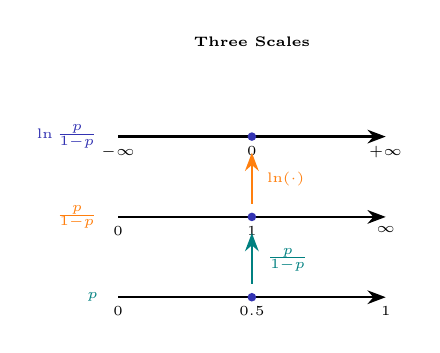
\begin{tikzpicture}[scale=0.68]
% Probability scale
\draw[-{Stealth}, thick] (0,0) -- (5,0);
\node[font=\tiny\bfseries, above] at (2.5,4.5) {Three Scales};
\node[font=\tiny, below] at (0,0) {$0$};
\node[font=\tiny, below] at (2.5,0) {$0.5$};
\node[font=\tiny, below] at (5,0) {$1$};
\node[font=\tiny\bfseries, dfteal, left] at (-0.2,0) {$p$};
% Odds scale
\draw[-{Stealth}, thick] (0,1.5) -- (5,1.5);
\node[font=\tiny, below] at (0,1.5) {$0$};
\node[font=\tiny, below] at (2.5,1.5) {$1$};
\node[font=\tiny, below] at (5,1.5) {$\infty$};
\node[font=\tiny\bfseries, mlorange, left] at (-0.2,1.5) {$\frac{p}{1-p}$};
% Log-odds scale
\draw[-{Stealth}, thick] (0,3.0) -- (5,3.0);
\node[font=\tiny, below] at (0,3.0) {$-\infty$};
\node[font=\tiny, below] at (2.5,3.0) {$0$};
\node[font=\tiny, below] at (5,3.0) {$+\infty$};
\node[font=\tiny\bfseries, mlpurple, left] at (-0.2,3.0) {$\ln\frac{p}{1-p}$};
% Arrows connecting scales
\draw[-{Stealth}, dfteal, thick] (2.5,0.25) -- (2.5,1.2);
\draw[-{Stealth}, mlorange, thick] (2.5,1.75) -- (2.5,2.7);
\node[font=\tiny, right, dfteal] at (2.6,0.7) {$\frac{p}{1-p}$};
\node[font=\tiny, right, mlorange] at (2.6,2.2) {$\ln(\cdot)$};
% Highlight p=0.5
\fill[mlpurple] (2.5,0) circle (0.08);
\fill[mlpurple] (2.5,1.5) circle (0.08);
\fill[mlpurple] (2.5,3.0) circle (0.08);
\end{tikzpicture}
\end{columns}

\bottomnote{Coefficients are additive in log-odds, multiplicative in odds -- this drives the odds-ratio interpretation}
\end{frame}

%% ================================================================
%% FRAME 7: Maximum Likelihood Estimation
%% ================================================================
\begin{frame}[t]{How Does Maximum Likelihood Find the Best Coefficients?}
\begin{columns}[T]
\column{0.55\textwidth}
\small
\textbf{The Likelihood Function}

\scriptsize
For $n$ observations with labels $y_i \in \{0,1\}$ and predicted probabilities $p_i = \sigma(\mathbf{w}^\top\mathbf{x}_i)$:

\vspace{2mm}
\textbf{Likelihood:}
$\displaystyle L(\mathbf{w}) = \prod_{i=1}^{n} p_i^{\,y_i}(1-p_i)^{1-y_i}$

\vspace{2mm}
\textbf{Log-likelihood:}
$\displaystyle \ell(\mathbf{w}) = \sum_{i=1}^{n}\bigl[y_i \ln p_i + (1-y_i)\ln(1-p_i)\bigr]$

\vspace{2mm}
\textbf{Why MLE, not OLS?} OLS assumes Gaussian errors. Binary outcomes follow a Bernoulli distribution, so MLE is the natural estimator.

\begin{block}{Insight}
\scriptsize MLE maximizes the probability of observing the actual data. There is no closed-form solution -- we must use iterative optimization.
\end{block}

\column{0.42\textwidth}
\footnotesize
\vspace{4mm}
\fcolorbox{mlpurple}{mllavender4}{\parbox{0.88\columnwidth}{%
\textbf{Key insight:}

\vspace{2mm}
Taking the log converts the product into a sum, making derivatives tractable.

\vspace{2mm}
The log-likelihood is \textbf{concave} in $\mathbf{w}$, guaranteeing a unique global maximum.

\vspace{2mm}
\textbf{No closed form:} unlike linear regression, $\hat{\mathbf{w}}_{\text{MLE}}$ cannot be written as $(X^\top X)^{-1}X^\top y$.
}}
\end{columns}

\bottomnote{The Bernoulli likelihood is the starting point -- everything (gradient, Hessian, inference) derives from it}
\end{frame}

%% ================================================================
%% FRAME 8: Cross-Entropy Loss (Chart)
%% ================================================================
\begin{frame}[t]{Why Does Cross-Entropy Loss Guarantee a Global Optimum?}
\begin{columns}[T]
\column{0.55\textwidth}
\small
\textbf{Binary Cross-Entropy}

\begin{compactlist}
\item \textbf{What you see:} The loss curves for $y=1$ and $y=0$ as a function of predicted $p$
\item \textbf{Key pattern:} Loss explodes as the prediction moves away from the true label
\item \textbf{Takeaway:} Confident wrong predictions are penalized far more than uncertain ones
\end{compactlist}

\vspace{1mm}
\scriptsize
$\displaystyle J(\mathbf{w}) = -\frac{1}{n}\sum_{i=1}^{n}\bigl[y_i \ln p_i + (1-y_i)\ln(1-p_i)\bigr]$

\vspace{1mm}
This is the negative log-likelihood divided by $n$. Minimizing $J$ = maximizing $\ell$.

\begin{block}{Insight}
\scriptsize Cross-entropy is convex in $\mathbf{w}$ (since $-\ell$ is convex). Every local minimum is the global minimum. No random restarts needed.
\end{block}

\column{0.42\textwidth}
\vspace{2mm}
\includegraphics[width=\textwidth]{03_log_loss/chart.pdf}
\end{columns}

\bottomnote{Convexity of the loss is the key theoretical advantage of logistic regression over neural networks}
\end{frame}

%% ================================================================
%% FRAME 9: Gradient in Matrix Form
%% ================================================================
\begin{frame}[t]{What Does the Gradient Look Like in Matrix Form?}
\begin{columns}[T]
\column{0.55\textwidth}
\small
\textbf{Deriving the Gradient}

\scriptsize
Apply the chain rule to the log-likelihood:

\vspace{2mm}
\textbf{Scalar form:}
$\displaystyle \frac{\partial \ell}{\partial w_j} = \sum_{i=1}^{n}(y_i - p_i)\,x_{ij}$

\vspace{2mm}
\textbf{Matrix form:}
$\displaystyle \nabla_{\mathbf{w}} \ell = \mathbf{X}^\top(\mathbf{y} - \mathbf{p})$

\vspace{2mm}
\textbf{For minimizing the loss (negative log-likelihood):}

$\displaystyle \nabla_{\mathbf{w}} J = \frac{1}{n}\mathbf{X}^\top(\mathbf{p} - \mathbf{y})$

\vspace{2mm}
\fcolorbox{mlpurple}{mllavender4}{\parbox{0.92\columnwidth}{%
\textbf{Compare to linear regression:} $\nabla J_{\text{LR}} = \frac{1}{n}\mathbf{X}^\top(\mathbf{X}\mathbf{w} - \mathbf{y})$.

The only difference: $\mathbf{p} = \sigma(\mathbf{X}\mathbf{w})$ replaces $\mathbf{X}\mathbf{w}$.
}}

\begin{block}{Insight}
\scriptsize The gradient has the same ``residual times features'' form as linear regression. The sigmoid is hidden inside $\mathbf{p}$.
\end{block}

\column{0.42\textwidth}
\footnotesize
\vspace{4mm}
\fcolorbox{dfteal}{dfteal!8}{\parbox{0.88\columnwidth}{%
\textbf{Chain rule steps:}

\vspace{2mm}
1. $\frac{\partial \ell}{\partial p_i} = \frac{y_i}{p_i} - \frac{1-y_i}{1-p_i}$

\vspace{2mm}
2. $\frac{\partial p_i}{\partial z_i} = p_i(1-p_i)$

\vspace{2mm}
3. $\frac{\partial z_i}{\partial w_j} = x_{ij}$

\vspace{2mm}
4. Combine: $\frac{\partial \ell}{\partial w_j} = (y_i - p_i)\,x_{ij}$

\vspace{2mm}
The $p_i(1-p_i)$ cancels, yielding a clean form.
}}
\end{columns}

\bottomnote{Setting the gradient to zero gives the score equations -- solved iteratively by gradient descent or Newton's method}
\end{frame}

%% ================================================================
%% FRAME 10: Gradient Descent
%% ================================================================
\begin{frame}[t]{How Does Gradient Descent Update the Weights?}
\begin{columns}[T]
\column{0.55\textwidth}
\small
\textbf{The Update Rule}

\scriptsize
$\displaystyle \mathbf{w}^{(t+1)} = \mathbf{w}^{(t)} - \eta\,\frac{1}{n}\mathbf{X}^\top\!\bigl(\sigma(\mathbf{X}\mathbf{w}^{(t)}) - \mathbf{y}\bigr)$

\vspace{2mm}
\begin{compactlist}
\item $\eta$ = learning rate (too large: diverge; too small: slow)
\item Convergence guaranteed for convex loss with appropriate $\eta$
\item \textbf{Feature standardization} essential: unscaled features create elongated contours, slowing convergence
\end{compactlist}

\vspace{1mm}
\scriptsize
\textbf{Variants:} Batch (full data), mini-batch (subset), stochastic (single sample). Scikit-learn uses L-BFGS by default.

\begin{block}{Insight}
\scriptsize Gradient descent follows the steepest downhill direction. On elongated loss surfaces (unscaled features), it zigzags. Standardize first.
\end{block}

\column{0.42\textwidth}
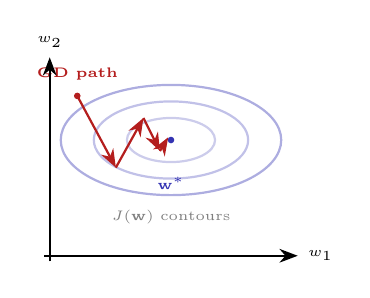
\begin{tikzpicture}[scale=0.7]
% Contour ellipses (loss surface)
\draw[mllavender, thick] (2,2) ellipse (2.0 and 1.0);
\draw[mllavender2, thick] (2,2) ellipse (1.4 and 0.7);
\draw[mllavender3, thick] (2,2) ellipse (0.8 and 0.4);
\fill[mlpurple] (2,2) circle (0.06);
\node[font=\tiny, mlpurple, below] at (2,1.5) {$\mathbf{w}^*$};
% GD path (zigzag)
\fill[dfred] (0.3,2.8) circle (0.06);
\draw[-{Stealth}, dfred, thick] (0.3,2.8) -- (1.0,1.5);
\draw[-{Stealth}, dfred, thick] (1.0,1.5) -- (1.5,2.4);
\draw[-{Stealth}, dfred, thick] (1.5,2.4) -- (1.8,1.8);
\draw[-{Stealth}, dfred, thick] (1.8,1.8) -- (1.95,2.05);
\node[font=\tiny\bfseries, dfred] at (0.3,3.2) {GD path};
% Labels
\node[font=\tiny, mlgray] at (2,0.6) {$J(\mathbf{w})$ contours};
\draw[-{Stealth}, thick] (-0.3,-0.1) -- (4.3,-0.1) node[right, font=\tiny] {$w_1$};
\draw[-{Stealth}, thick] (-0.2,-0.2) -- (-0.2,3.5) node[above, font=\tiny] {$w_2$};
\end{tikzpicture}
\end{columns}

\bottomnote{Convergence rate: $O(1/t)$ for gradient descent vs.\ quadratic for Newton -- but GD avoids Hessian inversion}
\end{frame}

%% ================================================================
%% FRAME 11: Newton-Raphson / IRLS
%% ================================================================
\begin{frame}[t]{Why Do Statisticians Prefer Newton-Raphson Over Gradient Descent?}
\begin{columns}[T]
\column{0.55\textwidth}
\small
\textbf{Newton-Raphson (IRLS)}

\scriptsize
The Hessian of the log-likelihood:

$\displaystyle \mathbf{H} = -\mathbf{X}^\top \mathbf{S}\,\mathbf{X}$

where $\mathbf{S} = \text{diag}(p_i(1-p_i))$ is the weight matrix.

\vspace{2mm}
\textbf{Newton update:}
$\displaystyle \mathbf{w}^{(t+1)} = \mathbf{w}^{(t)} - \mathbf{H}^{-1}\nabla\ell$

\vspace{2mm}
\begin{compactlist}
\item Converges in 5--10 iterations (quadratic rate)
\item Equivalent to Iteratively Reweighted Least Squares (IRLS)
\item Default in R's \texttt{glm()} and Python's \texttt{statsmodels}
\end{compactlist}

\begin{block}{Insight}
\scriptsize Newton uses curvature information (Hessian) to take optimal steps. The cost is $O(d^3)$ per iteration for the matrix inversion.
\end{block}

\column{0.42\textwidth}
\footnotesize
\vspace{2mm}
\fcolorbox{dfteal}{dfteal!8}{\parbox{0.88\columnwidth}{%
\textbf{IRLS Pseudocode:}

\vspace{1mm}
\scriptsize
1. Initialize $\mathbf{w}^{(0)} = \mathbf{0}$

2. \textbf{Repeat} until convergence:

\quad a. $\mathbf{p} = \sigma(\mathbf{X}\mathbf{w}^{(t)})$

\quad b. $\mathbf{S} = \text{diag}(p_i(1-p_i))$

\quad c. $\mathbf{z} = \mathbf{X}\mathbf{w}^{(t)} + \mathbf{S}^{-1}(\mathbf{y}-\mathbf{p})$

\quad d. $\mathbf{w}^{(t+1)} = (\mathbf{X}^\top\mathbf{S}\mathbf{X})^{-1}\mathbf{X}^\top\mathbf{S}\mathbf{z}$

3. Return $\hat{\mathbf{w}}$

\vspace{1mm}
Step (d) is a weighted least squares solve with weights $\mathbf{S}$.
}}
\end{columns}

\bottomnote{IRLS converges quadratically: each iteration roughly doubles the number of correct digits in $\hat{\mathbf{w}}$}
\end{frame}

%% === SECTION 2: DECISION BOUNDARIES ===

%% ================================================================
%% FRAME 12: Decision Boundary (Chart)
%% ================================================================
\begin{frame}[t]{Where Does the Decision Boundary Live in Feature Space?}
\begin{columns}[T]
\column{0.55\textwidth}
\small
\textbf{The Linear Boundary}

\begin{compactlist}
\item \textbf{What you see:} A line (or hyperplane) separating two classes in feature space
\item \textbf{Key pattern:} Points far from the boundary have high-confidence predictions
\item \textbf{Takeaway:} The boundary is where $\mathbf{w}^\top\mathbf{x}+b=0$, i.e., $P=0.5$
\end{compactlist}

\vspace{1mm}
\scriptsize
The threshold $P=0.5$ is the default, but banks often use $P=0.3$ or lower for credit scoring where the cost of a missed default is high.

\begin{block}{Insight}
\scriptsize The model draws a linear boundary. The threshold shifts the boundary parallel to itself -- choosing it is a business decision, not a statistical one.
\end{block}

\column{0.42\textwidth}
\vspace{2mm}
\includegraphics[width=\textwidth]{02_decision_boundary/chart.pdf}
\end{columns}

\bottomnote{$\mathbf{w}^\top\mathbf{x}+b=0$ defines a hyperplane in $\mathbb{R}^d$; the normal vector is $\mathbf{w}$}
\end{frame}

%% ================================================================
%% FRAME 13: Non-Linear Patterns / Polynomial Features
%% ================================================================
\begin{frame}[t]{How Can a Linear Model Capture Non-Linear Patterns?}
\begin{columns}[T]
\column{0.55\textwidth}
\small
\textbf{Feature Engineering for Non-Linearity}

\begin{compactlist}
\item \textbf{Polynomial features:} Add $x^2$, $x_1 x_2$ to make the boundary curved
\item \textbf{Interaction terms:} Capture joint effects (e.g., income $\times$ debt)
\item \textbf{Binning / splines:} Piecewise-linear approximation of non-linear effects
\end{compactlist}

\vspace{1mm}
\scriptsize
The model remains linear \emph{in its parameters} -- the boundary is non-linear only in the original feature space.

\begin{block}{Insight}
\scriptsize Feature engineering is how logistic regression competes with non-linear models. The trade-off: flexibility vs.\ overfitting and loss of interpretability.
\end{block}

\column{0.42\textwidth}
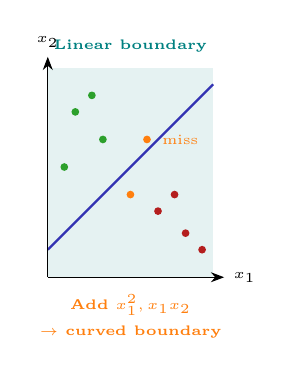
\begin{tikzpicture}[scale=0.7]
% Left: linear boundary
\node[font=\tiny\bfseries, dfteal] at (1.5,4.2) {Linear boundary};
\fill[dfteal!10] (0,0) -- (0,3.8) -- (3,3.8) -- (3,0) -- cycle;
% Data points
\foreach \x/\y in {0.5/3.0, 1.0/2.5, 0.8/3.3, 0.3/2.0} {
  \fill[mlgreen] (\x,\y) circle (0.07);
}
\foreach \x/\y in {2.5/0.8, 2.0/1.2, 2.8/0.5, 2.3/1.5} {
  \fill[dfred] (\x,\y) circle (0.07);
}
% Linear boundary
\draw[mlpurple, thick] (0,0.5) -- (3,3.5);
% Misclassified points
\fill[mlorange] (1.5,1.5) circle (0.07);
\fill[mlorange] (1.8,2.5) circle (0.07);
\node[font=\tiny, mlorange, right] at (1.9,2.5) {miss};
% Axes
\draw[-{Stealth}] (0,0) -- (3.2,0) node[right, font=\tiny] {$x_1$};
\draw[-{Stealth}] (0,0) -- (0,4.0) node[above, font=\tiny] {$x_2$};
% Curved boundary (below)
\node[font=\tiny\bfseries, mlorange] at (1.5,-0.5) {Add $x_1^2, x_1 x_2$};
\node[font=\tiny\bfseries, mlorange] at (1.5,-1.0) {$\to$ curved boundary};
\end{tikzpicture}
\end{columns}

\bottomnote{Polynomial features of degree $d$ with $p$ variables create $\binom{p+d}{d}$ features -- growth is combinatorial}
\end{frame}

%% ================================================================
%% FRAME 14: Multiclass (Softmax)
%% ================================================================
\begin{frame}[t]{What Changes When There Are More Than Two Classes?}
\begin{columns}[T]
\column{0.55\textwidth}
\small
\textbf{Softmax Regression}

\scriptsize
For $K$ classes, each has its own weight vector $\mathbf{w}_k$:

\vspace{2mm}
$\displaystyle P(y=k \mid \mathbf{x}) = \frac{\exp(\mathbf{w}_k^\top \mathbf{x})}{\sum_{j=1}^{K}\exp(\mathbf{w}_j^\top \mathbf{x})}$

\vspace{2mm}
\begin{compactlist}
\item Probabilities sum to 1 across all classes
\item Loss: categorical cross-entropy $= -\sum_k y_k \ln p_k$
\item \textbf{One-vs-Rest (OvR):} fit $K$ binary classifiers, cheaper but less principled
\end{compactlist}

\vspace{1mm}
\scriptsize
For credit scoring, the outcome is usually binary (default/no-default), so softmax is rare. But multi-class extensions appear in rating migration models (AAA, AA, A, BBB, \ldots).

\begin{block}{Insight}
\scriptsize Softmax generalizes the sigmoid to $K$ classes. When $K=2$, softmax reduces exactly to the standard sigmoid.
\end{block}

\column{0.42\textwidth}
\footnotesize
\vspace{4mm}
\fcolorbox{mlpurple}{mllavender4}{\parbox{0.88\columnwidth}{%
\textbf{Softmax vs.\ Sigmoid:}

\vspace{2mm}
\scriptsize
$K=2$: \; $\frac{e^{w_1^\top x}}{e^{w_1^\top x}+e^{w_2^\top x}}$

\vspace{1mm}
$= \frac{1}{1+e^{-(w_1-w_2)^\top x}} = \sigma(\Delta w^\top x)$

\vspace{3mm}
\textbf{One-vs-Rest:}

Fit $K$ independent binary models. Faster to train but predictions may not sum to 1.

\vspace{3mm}
\textbf{In practice:} Scikit-learn uses OvR by default; statsmodels uses multinomial logit.
}}
\end{columns}

\bottomnote{Softmax is the canonical link for the multinomial distribution -- the multi-class generalization of the logit}
\end{frame}

%% === SECTION 3: STATISTICAL INFERENCE ===

%% ================================================================
%% FRAME 15: Standard Errors from Hessian
%% ================================================================
\begin{frame}[t]{How Certain Are We About Each Coefficient?}
\begin{columns}[T]
\column{0.55\textwidth}
\small
\textbf{Standard Errors from the Hessian}

\scriptsize
The Fisher information matrix equals the negative expected Hessian:

\vspace{2mm}
$\displaystyle \mathcal{I}(\mathbf{w}) = \mathbf{X}^\top\mathbf{S}\,\mathbf{X}$
\quad where $\mathbf{S}=\text{diag}(p_i(1-p_i))$.

\vspace{2mm}
The variance-covariance matrix of $\hat{\mathbf{w}}$:
$\displaystyle \text{Var}(\hat{\mathbf{w}}) = \mathcal{I}(\hat{\mathbf{w}})^{-1} = (\mathbf{X}^\top\hat{\mathbf{S}}\,\mathbf{X})^{-1}$

\vspace{2mm}
Standard error of coefficient $j$:
$\displaystyle \text{SE}(\hat{w}_j) = \sqrt{[\mathcal{I}^{-1}]_{jj}}$

\vspace{1mm}
\begin{compactlist}
\item More data $\Rightarrow$ larger $\mathcal{I}$ $\Rightarrow$ smaller SE
\item Correlated features $\Rightarrow$ inflated SE (multicollinearity)
\end{compactlist}

\begin{block}{Insight}
\scriptsize The Hessian serves double duty: it accelerates optimization (Newton) and quantifies uncertainty (standard errors). Both come from the same matrix.
\end{block}

\column{0.42\textwidth}
\footnotesize
\vspace{4mm}
\fcolorbox{dfteal}{dfteal!8}{\parbox{0.88\columnwidth}{%
\textbf{Worked example:}

\vspace{2mm}
\scriptsize
Credit scoring model with 3 features:

\vspace{1mm}
\begin{tabular}{@{}lcc@{}}
Feature & $\hat{w}$ & SE \\
\midrule
Income & $0.50$ & $0.12$ \\
Debt ratio & $-1.20$ & $0.25$ \\
Employment & $0.30$ & $0.15$ \\
\end{tabular}

\vspace{2mm}
Income: $0.50/0.12 = 4.17 > 1.96$ \checkmark

Debt: $1.20/0.25 = 4.80 > 1.96$ \checkmark

Employment: $0.30/0.15 = 2.00 > 1.96$ \checkmark

\vspace{1mm}
All three are significant at $\alpha=0.05$.
}}
\end{columns}

\bottomnote{Asymptotic normality: $\hat{w}_j \;\dot\sim\; N(w_j,\, [\mathcal{I}^{-1}]_{jj})$ for large $n$}
\end{frame}

%% ================================================================
%% FRAME 16: Wald Test
%% ================================================================
\begin{frame}[t]{Is This Feature Significant? (Wald Test)}
\begin{columns}[T]
\column{0.55\textwidth}
\small
\textbf{The Wald Test}

\scriptsize
\textbf{Null hypothesis:} $H_0\!: w_j = 0$ (feature $j$ has no effect)

\vspace{2mm}
\textbf{Test statistic:}
$\displaystyle z = \frac{\hat{w}_j}{\text{SE}(\hat{w}_j)} \;\dot\sim\; N(0,1)$

\vspace{2mm}
\textbf{Decision rule:} Reject $H_0$ if $|z| > z_{\alpha/2}$ (e.g., $|z|>1.96$ at 5\%).

\vspace{2mm}
\textbf{Confidence interval:}
$\hat{w}_j \pm z_{\alpha/2}\cdot\text{SE}(\hat{w}_j)$

\vspace{2mm}
\begin{compactlist}
\item For odds ratios: exponentiate the CI endpoints
\item Wald test is fast (no model refitting) but unreliable for large $|\hat{w}_j|$
\item Hauck--Donner effect: Wald becomes conservative when coefficients are large
\end{compactlist}

\begin{block}{Insight}
\scriptsize The Wald test answers: ``Is this coefficient significantly different from zero?'' For comparing nested models, use the more powerful LRT instead.
\end{block}

\column{0.42\textwidth}
\footnotesize
\vspace{4mm}
\fcolorbox{mlpurple}{mllavender4}{\parbox{0.88\columnwidth}{%
\textbf{Worked example:}

\vspace{2mm}
\scriptsize
Feature: number of late payments

$\hat{w} = 0.85$, \; $\text{SE} = 0.18$

$z = 0.85 / 0.18 = 4.72$

$p\text{-value} < 0.001$

\vspace{2mm}
\textbf{95\% CI for $w$:}

$0.85 \pm 1.96 \times 0.18 = [0.50,\; 1.20]$

\vspace{2mm}
\textbf{95\% CI for OR:}

$[e^{0.50},\; e^{1.20}] = [1.65,\; 3.32]$

\vspace{2mm}
Each additional late payment multiplies default odds by 1.65--3.32.
}}
\end{columns}

\bottomnote{The Wald test is the default in statsmodels and R's summary.glm -- but LRT is more reliable for small samples}
\end{frame}

%% ================================================================
%% FRAME 17: Likelihood Ratio Test + AIC/BIC
%% ================================================================
\begin{frame}[t]{Does Adding These Features Actually Improve the Model?}
\begin{columns}[T]
\column{0.55\textwidth}
\small
\textbf{Likelihood Ratio Test (LRT)}

\scriptsize
\textbf{Setup:} Compare a reduced model (fewer features) vs.\ a full model.

\vspace{2mm}
$\displaystyle \Lambda = -2\bigl[\ell(\text{reduced}) - \ell(\text{full})\bigr] \;\dot\sim\; \chi^2_{q}$

where $q$ = number of additional parameters in the full model.

\vspace{2mm}
\textbf{Example:} Adding 3 credit bureau features:

$\Lambda = -2[-1250 - (-1220)] = 60$, \; $q=3$

$\chi^2_3$ critical value at 5\% = $7.81$. Since $60 \gg 7.81$, the bureau features significantly improve the model.

\vspace{1mm}
\begin{compactlist}
\item LRT is more powerful than Wald for multiple coefficients
\item Requires fitting both models (more computation)
\end{compactlist}

\begin{block}{Insight}
\scriptsize LRT asks: ``Does the data support the added complexity?'' It is the gold standard for nested model comparison in regulatory settings.
\end{block}

\column{0.42\textwidth}
\footnotesize
\vspace{4mm}
\fcolorbox{dfteal}{dfteal!8}{\parbox{0.88\columnwidth}{%
\textbf{AIC and BIC:}

\vspace{2mm}
\scriptsize
For non-nested model comparison:

\vspace{1mm}
$\text{AIC} = -2\ell + 2k$

$\text{BIC} = -2\ell + k\ln n$

\vspace{2mm}
where $k$ = number of parameters, $n$ = sample size.

\vspace{2mm}
\textbf{BIC penalizes more} for large $n$ (when $\ln n > 2$, i.e., $n > 8$).

\vspace{2mm}
\textbf{Rule:} BIC preferred for regulatory models (stronger parsimony).

\vspace{2mm}
Lower is better for both. $\Delta > 10$ is strong evidence.
}}
\end{columns}

\bottomnote{Deviance = $-2\ell$; the LRT statistic is the difference in deviances between nested models}
\end{frame}

%% ================================================================
%% FRAME 18: McFadden R-squared
%% ================================================================
\begin{frame}[t]{How Do You Choose Between Two Non-Nested Models?}
\begin{columns}[T]
\column{0.55\textwidth}
\small
\textbf{Goodness-of-Fit Measures}

\scriptsize
\textbf{McFadden pseudo-$R^2$:}
$\displaystyle R^2_{\text{McF}} = 1 - \frac{\ell(\text{model})}{\ell(\text{null})}$

\vspace{2mm}
where $\ell(\text{null})$ = log-likelihood of intercept-only model.

\vspace{2mm}
\begin{compactlist}
\item Values 0.2--0.4 represent excellent fit (not comparable to OLS $R^2$)
\item Adjusted version: $R^2_{\text{adj}} = 1 - \frac{\ell(\text{model}) - k}{\ell(\text{null})}$
\end{compactlist}

\vspace{2mm}
\textbf{Hosmer--Lemeshow test:} Group predicted probabilities into deciles, compare observed vs.\ expected counts with $\chi^2$ test.

\vspace{1mm}
\begin{block}{Insight}
\scriptsize McFadden $R^2$ measures improvement over the null model. AIC/BIC are better for model selection; pseudo-$R^2$ is better for reporting overall explanatory power.
\end{block}

\column{0.42\textwidth}
\footnotesize
\vspace{2mm}
\begin{tabular}{@{}l c c@{}}
\toprule
\textbf{Measure} & \textbf{Range} & \textbf{Use} \\
\midrule
\rowcolor{mllavender4}
McFadden $R^2$ & $[0,1)$ & Overall fit \\
AIC & $\mathbb{R}^+$ & Model select \\
\rowcolor{mllavender4}
BIC & $\mathbb{R}^+$ & Regulatory \\
Deviance & $\mathbb{R}^+$ & LRT input \\
\rowcolor{mllavender4}
H--L test & $p$-value & Calibration \\
Brier score & $[0,1]$ & Probability \\
\bottomrule
\end{tabular}

\vspace{3mm}
\fcolorbox{mlpurple}{mllavender4}{\parbox{0.88\columnwidth}{%
\scriptsize\textbf{Rule of thumb:}

McFadden $R^2 \approx 0.2$ is already a well-fitting model. Do not compare to OLS $R^2$ values.
}}
\end{columns}

\bottomnote{No single metric suffices -- report deviance, AIC, pseudo-$R^2$, and a calibration test together}
\end{frame}

%% === SECTION 4: EVALUATION METRICS ===

%% ================================================================
%% FRAME 19: ROC Curve (Chart)
%% ================================================================
\begin{frame}[t]{How Do You Measure Discrimination Across All Thresholds?}
\begin{columns}[T]
\column{0.55\textwidth}
\small
\textbf{The ROC Curve}

\begin{compactlist}
\item \textbf{What you see:} True Positive Rate vs.\ False Positive Rate at every threshold
\item \textbf{Key pattern:} The curve bows toward the top-left corner for good models
\item \textbf{Takeaway:} AUC summarizes discrimination power in a single number
\end{compactlist}

\vspace{1mm}
\scriptsize
\textbf{Interpretation:}
\begin{compactlist}
\item Diagonal = random classifier (AUC = 0.5)
\item Perfect classifier hugs the top-left corner (AUC = 1.0)
\item AUC = probability that a random positive ranks higher than a random negative
\end{compactlist}

\begin{block}{Insight}
\scriptsize The ROC curve shows the trade-off between catching defaults (TPR) and raising false alarms (FPR) at every possible threshold.
\end{block}

\column{0.42\textwidth}
\vspace{2mm}
\includegraphics[width=\textwidth]{04_roc_curve/chart.pdf}
\end{columns}

\bottomnote{ROC is threshold-invariant: it evaluates the model's ranking ability, not any specific cutoff}
\end{frame}

%% ================================================================
%% FRAME 20: AUC and Gini
%% ================================================================
\begin{frame}[t]{What Does AUC Really Mean, and What Is the Gini Coefficient?}
\begin{columns}[T]
\column{0.55\textwidth}
\small
\textbf{AUC and Gini}

\scriptsize
\textbf{AUC (Area Under the ROC Curve):}
\begin{compactlist}
\item $\text{AUC} = P(\text{score}(+) > \text{score}(-))$
\item Equivalent to the Wilcoxon--Mann--Whitney statistic
\end{compactlist}

\vspace{2mm}
\textbf{Gini coefficient:}
$\displaystyle \text{Gini} = 2 \times \text{AUC} - 1$

\vspace{2mm}
\textbf{KS statistic:} Maximum vertical distance between CDFs of positive and negative classes.

\begin{block}{Insight}
\scriptsize Gini is the industry standard in credit scoring. Gini $> 0.40$ is acceptable; Gini $> 0.60$ is good. These thresholds appear in Basel validation guidelines.
\end{block}

\column{0.42\textwidth}
\footnotesize
\vspace{2mm}
\begin{tabular}{@{}l c c@{}}
\toprule
\textbf{AUC} & \textbf{Gini} & \textbf{Quality} \\
\midrule
\rowcolor{mllavender4}
$0.50$ & $0.00$ & Random \\
$0.60$ & $0.20$ & Poor \\
\rowcolor{mllavender4}
$0.70$ & $0.40$ & Acceptable \\
$0.80$ & $0.60$ & Good \\
\rowcolor{mllavender4}
$0.90$ & $0.80$ & Excellent \\
$1.00$ & $1.00$ & Perfect \\
\bottomrule
\end{tabular}

\vspace{3mm}
\fcolorbox{dfteal}{dfteal!8}{\parbox{0.88\columnwidth}{%
\scriptsize\textbf{KS statistic:}

$\text{KS} = \max_t |F_+(t) - F_-(t)|$

KS $> 0.30$ is typical for good credit models. Reports the single threshold with maximum separation.
}}
\end{columns}

\bottomnote{Gini = $2 \times \text{AUC} - 1$: the standard discrimination metric reported to regulators under Basel~II/III}
\end{frame}

%% ================================================================
%% FRAME 21: Precision-Recall + Fraud (Chart)
%% ================================================================
\begin{frame}[t]{When Does ROC Lie, and Why Should You Use Precision-Recall?}
\begin{columns}[T]
\column{0.55\textwidth}
\small
\textbf{Precision-Recall for Imbalanced Data}

\begin{compactlist}
\item \textbf{What you see:} Precision vs.\ Recall curve -- how they trade off
\item \textbf{Key pattern:} High precision requires sacrificing recall (and vice versa)
\item \textbf{Takeaway:} PR curves are more informative than ROC when positives are rare
\end{compactlist}

\vspace{1mm}
\scriptsize
\textbf{Fraud detection example:} With 0.1\% fraud rate, a model predicting ``no fraud'' always achieves 99.9\% accuracy and AUC can still look impressive. But precision-recall reveals the model catches zero frauds.

\begin{block}{Insight}
\scriptsize ROC is optimistic on imbalanced data because TNR stays high. Precision-recall focuses on the rare class. Always report both in fraud and default prediction.
\end{block}

\column{0.42\textwidth}
\vspace{2mm}
\includegraphics[width=\textwidth]{05_precision_recall/chart.pdf}
\end{columns}

\bottomnote{Average Precision (AP) summarizes the PR curve; F1 = $2 \cdot \text{prec} \cdot \text{rec} / (\text{prec}+\text{rec})$ at a single threshold}
\end{frame}

%% ================================================================
%% FRAME 22: Confusion Matrix + Calibration (Chart)
%% ================================================================
\begin{frame}[t]{How Do You Know If Your Probabilities Are Truthful?}
\begin{columns}[T]
\column{0.55\textwidth}
\small
\textbf{Calibration and the Confusion Matrix}

\begin{compactlist}
\item \textbf{What you see:} Counts of TP, FP, TN, FN organized in a $2 \times 2$ matrix
\item \textbf{Key pattern:} Off-diagonal entries are errors; their costs differ in finance
\item \textbf{Takeaway:} A well-calibrated model means predicted $P=0.05$ matches observed 5\% default rate
\end{compactlist}

\vspace{1mm}
\scriptsize
\textbf{Brier score:} $\text{BS} = \frac{1}{n}\sum(p_i - y_i)^2$. Lower is better; $\text{BS}=0$ is perfect.

\textbf{Hosmer--Lemeshow:} Group predictions into deciles, test observed vs.\ expected with $\chi^2$.

\begin{block}{Insight}
\scriptsize Discrimination (AUC) and calibration are independent properties. A model can rank well but assign wrong probabilities. Credit scoring requires both.
\end{block}

\column{0.42\textwidth}
\vspace{2mm}
\includegraphics[width=\textwidth]{06_confusion_matrix/chart.pdf}
\end{columns}

\bottomnote{Calibration is critical for Basel PD: regulators require predicted PDs to match realized default rates}
\end{frame}

%% ================================================================
%% FRAME 23: Separation Problem
%% ================================================================
\begin{frame}[t]{What Could Go Wrong When Data Perfectly Separates the Classes?}
\begin{columns}[T]
\column{0.55\textwidth}
\small
\textbf{Complete and Quasi-Complete Separation}

\begin{compactlist}
\item If one feature perfectly predicts the outcome, the MLE does not exist
\item Coefficients diverge to $\pm\infty$ as the optimizer tries to make $p \to 0$ or $p \to 1$
\item Standard errors become infinite; Wald tests become meaningless
\end{compactlist}

\vspace{1mm}
\scriptsize
\textbf{Solutions:}
\begin{compactlist}
\item \textbf{Firth's penalized likelihood:} adds a bias correction term
\item \textbf{L2 regularization:} shrinks coefficients, prevents divergence
\item \textbf{Bayesian logistic regression:} prior on coefficients keeps them finite
\end{compactlist}

\begin{block}{Insight}
\scriptsize Separation is common in small samples or rare-event data (e.g., low-default portfolios). Always check for convergence warnings in your output.
\end{block}

\column{0.42\textwidth}
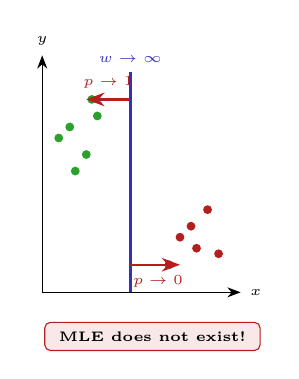
\begin{tikzpicture}[scale=0.7]
% Scatter plot with perfect separation
\foreach \x/\y in {0.5/3.0, 0.8/2.5, 0.3/2.8, 1.0/3.2, 0.6/2.2, 0.9/3.5} {
  \fill[mlgreen] (\x,\y) circle (0.08);
}
\foreach \x/\y in {2.5/1.0, 2.8/0.8, 3.0/1.5, 2.3/0.5, 2.7/1.2, 3.2/0.7} {
  \fill[dfred] (\x,\y) circle (0.08);
}
% Perfect separating line
\draw[mlpurple, very thick] (1.6,0) -- (1.6,4.0);
\node[font=\tiny, mlpurple, above] at (1.6,4.0) {$w \to \infty$};
% Arrows showing divergence
\draw[-{Stealth}, dfred, thick] (1.6,3.5) -- (0.8,3.5);
\draw[-{Stealth}, dfred, thick] (1.6,0.5) -- (2.5,0.5);
\node[font=\tiny, dfred] at (1.2,3.8) {$p \to 1$};
\node[font=\tiny, dfred] at (2.1,0.2) {$p \to 0$};
% Warning
\node[draw=dfred, fill=dfred!10, rounded corners=2pt,
      font=\tiny\bfseries, text width=2.5cm, align=center]
      at (2.0,-0.8) {MLE does not exist!};
% Axes
\draw[-{Stealth}] (0,0) -- (3.6,0) node[right, font=\tiny] {$x$};
\draw[-{Stealth}] (0,0) -- (0,4.3) node[above, font=\tiny] {$y$};
\end{tikzpicture}
\end{columns}

\bottomnote{Firth (1993): penalized likelihood reduces bias and handles separation -- implemented in R's \texttt{brglm2}}
\end{frame}

%% === SECTION 5: REGULARIZATION ===

%% ================================================================
%% FRAME 24: Regularization Motivation
%% ================================================================
\begin{frame}[t]{Why Would You Penalize Coefficients That Fit the Data Well?}
\begin{columns}[T]
\column{0.55\textwidth}
\small
\textbf{The Overfitting Problem}

\begin{compactlist}
\item With many features and limited data, MLE overfits: $\hat{w}_j$ become large
\item The model memorizes training noise instead of learning patterns
\item Regularization adds a penalty: $J_{\text{reg}} = J + \lambda\,R(\mathbf{w})$
\end{compactlist}

\vspace{1mm}
\scriptsize
\textbf{Bias-variance trade-off:}
\begin{compactlist}
\item $\lambda = 0$: no penalty, high variance (overfitting)
\item $\lambda \to \infty$: all coefficients shrunk to zero, high bias (underfitting)
\item Optimal $\lambda$: minimizes generalization error
\end{compactlist}

\begin{block}{Insight}
\scriptsize Regularization is not a hack -- it is the Bayesian perspective: the penalty corresponds to a prior belief that coefficients should be small.
\end{block}

\column{0.42\textwidth}
\footnotesize
\vspace{4mm}
\fcolorbox{mlpurple}{mllavender4}{\parbox{0.88\columnwidth}{%
\textbf{Regularized loss:}

\vspace{2mm}
\scriptsize
$J_{\text{reg}} = \underbrace{-\frac{1}{n}\sum\bigl[y_i\ln p_i + (1-y_i)\ln(1-p_i)\bigr]}_{\text{cross-entropy}}$

\vspace{1mm}
$\qquad + \;\underbrace{\lambda\,R(\mathbf{w})}_{\text{penalty}}$

\vspace{3mm}
The penalty $R(\mathbf{w})$ controls model complexity. Three choices: L1, L2, or Elastic Net.

\vspace{2mm}
\textbf{Note:} Scikit-learn uses $C = 1/\lambda$, so larger $C$ means \emph{less} regularization.
}}
\end{columns}

\bottomnote{Regularization strength $\lambda$ (or $C=1/\lambda$) is the most important hyperparameter in logistic regression}
\end{frame}

%% ================================================================
%% FRAME 25: L1 / L2 / Elastic Net
%% ================================================================
\begin{frame}[t]{Should You Shrink All Coefficients or Zero Some Out?}
\begin{columns}[T]
\column{0.55\textwidth}
\small
\textbf{Three Regularization Strategies}

\scriptsize
\textbf{L2 (Ridge):} $R(\mathbf{w}) = \frac{1}{2}\sum_j w_j^2$

Shrinks all coefficients toward zero but never exactly to zero.

\vspace{2mm}
\textbf{L1 (Lasso):} $R(\mathbf{w}) = \sum_j |w_j|$

Drives some coefficients exactly to zero $\Rightarrow$ automatic feature selection.

\vspace{2mm}
\textbf{Elastic Net:} $R(\mathbf{w}) = \alpha\sum_j |w_j| + \frac{1-\alpha}{2}\sum_j w_j^2$

Combines L1 sparsity with L2 stability. Parameter $\alpha$ controls the mix.

\begin{block}{Insight}
\scriptsize L1 is preferred when you suspect many irrelevant features. L2 is preferred when all features may contribute. Elastic Net is the safe default for credit scoring.
\end{block}

\column{0.42\textwidth}
\footnotesize
\vspace{2mm}
\begin{tabular}{@{}l c c c@{}}
\toprule
& \textbf{L2} & \textbf{L1} & \textbf{EN} \\
\midrule
\rowcolor{mllavender4}
Sparsity & No & Yes & Yes \\
Stability & High & Low & High \\
\rowcolor{mllavender4}
Groups & All & One & All \\
Solution & Unique & Not & Unique \\
\rowcolor{mllavender4}
Bayesian & Gaussian & Laplace & Mix \\
\bottomrule
\end{tabular}

\vspace{3mm}
\fcolorbox{dfteal}{dfteal!8}{\parbox{0.88\columnwidth}{%
\scriptsize\textbf{Geometric view:}

L2 penalty = circle constraint.

L1 penalty = diamond constraint.

Diamond corners touch axes $\Rightarrow$ sparse solutions.
}}
\end{columns}

\bottomnote{Elastic Net with $\alpha=0.5$ is a robust default; L1 alone can be unstable with correlated features}
\end{frame}

%% ================================================================
%% FRAME 26: Lambda Selection via CV
%% ================================================================
\begin{frame}[t]{How Do You Choose the Regularization Strength?}
\begin{columns}[T]
\column{0.55\textwidth}
\small
\textbf{Cross-Validation for $\lambda$ (or $C$)}

\scriptsize
\begin{compactlist}
\item Split data into $K$ folds (typically $K=5$ or $10$)
\item For each candidate $C$ value, train on $K-1$ folds, evaluate on the held-out fold
\item Average the metric (log-loss or AUC) across folds
\item Select $C$ that maximizes average performance
\end{compactlist}

\vspace{2mm}
\textbf{In scikit-learn:}
\texttt{LogisticRegressionCV(Cs=20, cv=5, scoring='roc\_auc')}

Automatically searches 20 values of $C$ on a log scale.

\vspace{2mm}
\textbf{One-SE rule:} Choose the simplest model within one standard error of the best CV score. This promotes parsimony.

\begin{block}{Insight}
\scriptsize Never tune $\lambda$ on the test set. Cross-validation provides an unbiased estimate of generalization performance for each candidate.
\end{block}

\column{0.42\textwidth}
\footnotesize
\vspace{4mm}
\fcolorbox{mlpurple}{mllavender4}{\parbox{0.88\columnwidth}{%
\textbf{CV procedure:}

\vspace{2mm}
\scriptsize
1. Define grid: $C \in \{10^{-4}, \ldots, 10^{4}\}$

2. For each $C$:

\quad For each fold $k=1,\ldots,K$:

\quad\quad Train on folds $\neq k$

\quad\quad Score on fold $k$

\quad Average scores $\to \overline{S}(C)$

3. Pick $C^* = \arg\max_C \overline{S}(C)$

4. Refit on all data with $C^*$

\vspace{2mm}
\textbf{Stratified CV} ensures each fold has the same class ratio -- critical for imbalanced data.
}}
\end{columns}

\bottomnote{LogisticRegressionCV is 10x faster than GridSearchCV because it warm-starts along the regularization path}
\end{frame}

%% === SECTION 6: FINANCE APPLICATION ===

%% ================================================================
%% FRAME 27: Basel Credit Scoring (Chart)
%% ================================================================
\begin{frame}[t]{How Do Banks Turn Logistic Regression Into Credit Scores?}
\begin{columns}[T]
\column{0.55\textwidth}
\small
\textbf{Scorecard Construction}

\begin{compactlist}
\item \textbf{What you see:} The decision flowchart from features to approval/denial
\item \textbf{Key pattern:} Each step adds interpretability and auditability
\item \textbf{Takeaway:} Scorecards convert log-odds to points using a linear transform
\end{compactlist}

\vspace{1mm}
\scriptsize
\textbf{Points-to-Double-the-Odds (PDO):}

$\text{Score} = \text{Offset} + \text{Factor} \times \ln(\text{odds})$

where Factor $= \text{PDO}/\ln(2)$.

If PDO=20 and base odds 50:1 at score 600, each 20-point drop doubles the default odds.

\begin{block}{Insight}
\scriptsize Basel~II/III requires banks to estimate PD for each rating grade. Logistic regression is the workhorse because every coefficient is auditable and every PD is calibrated.
\end{block}

\column{0.42\textwidth}
\vspace{2mm}
\includegraphics[width=\textwidth]{07_decision_flowchart/chart.pdf}
\end{columns}

\bottomnote{IRB approach: PD must be validated annually with backtesting, benchmarking, and discrimination analysis}
\end{frame}

%% ================================================================
%% FRAME 28: Feature Engineering + PD Worked Example
%% ================================================================
\begin{frame}[t]{What Features Do Credit Scorecards Actually Use?}
\begin{columns}[T]
\column{0.55\textwidth}
\small
\textbf{Feature Engineering for Credit}

\scriptsize
\textbf{Weight of Evidence (WoE) encoding:}

$\text{WoE}_j = \ln\!\left(\frac{\%\text{non-default}_j}{\%\text{default}_j}\right)$

Transforms categorical features into a monotonic scale aligned with log-odds.

\vspace{2mm}
\textbf{Common credit features:}
\begin{compactlist}
\item Debt-to-income ratio (DTI)
\item Employment stability (years)
\item Bureau delinquency count
\item Credit utilization ratio
\item Time since last delinquency
\end{compactlist}

\begin{block}{Insight}
\scriptsize WoE encoding is the standard in credit scoring because it preserves the linear relationship with log-odds and handles missing values naturally.
\end{block}

\column{0.42\textwidth}
\footnotesize
\vspace{2mm}
\fcolorbox{dfteal}{dfteal!8}{\parbox{0.88\columnwidth}{%
\textbf{Worked example:}

\vspace{2mm}
\scriptsize
Applicant profile:

\begin{tabular}{@{}lc@{}}
Feature & Value \\
\midrule
Income & \$55k \\
DTI & 0.32 \\
Employment & 6 years \\
Late payments & 1 \\
Utilization & 0.45 \\
\end{tabular}

\vspace{2mm}
$z = -2.1 + 0.5(0.55) + (-1.2)(0.32)$

$\quad + 0.3(0.6) + 0.85(1) + (-0.4)(0.45)$

$= -2.1 + 0.275 - 0.384 + 0.18$

$\quad + 0.85 - 0.18 = -1.359$

\vspace{1mm}
$\text{PD} = \sigma(-1.359) = 0.204$

\vspace{1mm}
\textbf{Decision:} PD = 20.4\%, above the 15\% cutoff $\to$ \textcolor{dfred}{Deny}
}}
\end{columns}

\bottomnote{PD estimation is the foundation: it feeds into EAD and LGD to compute Expected Loss = PD $\times$ EAD $\times$ LGD}
\end{frame}

%% ================================================================
%% FRAME 29: Stakeholder Map + Fairness
%% ================================================================
\begin{frame}[t]{Who Wins and Who Loses When Models Replace Loan Officers?}
\begin{columns}[T]
\column{0.55\textwidth}
\small
\textbf{Stakeholder Analysis}

\begin{compactlist}
\item \textbf{Winners:} Risk managers (calibrated PD), regulators (auditable model), applicants (consistent decisions)
\item \textbf{Losers:} Data scientists wanting complex models, branch managers (discretion reduced)
\end{compactlist}

\vspace{1mm}
\scriptsize
\textbf{Fairness considerations:}
\begin{compactlist}
\item Protected attributes (race, gender, age) must not be direct features
\item \textbf{Disparate impact:} Even without protected features, proxy variables can create bias
\item GDPR Article 22: right to explanation of automated decisions
\end{compactlist}

\begin{block}{Insight}
\scriptsize In regulated finance, interpretability is not optional -- it is a legal requirement under Basel~II/III and GDPR Article~22. LogReg is the compliance-friendly default.
\end{block}

\column{0.42\textwidth}
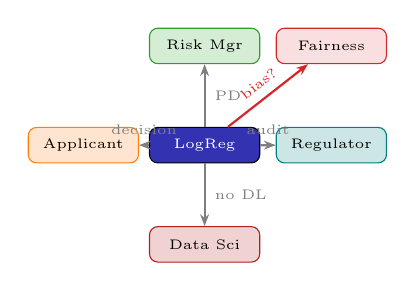
\begin{tikzpicture}[scale=0.7,
  actor/.style={draw, rounded corners=3pt, font=\tiny,
    minimum width=1.4cm, minimum height=0.45cm, align=center},
  arr/.style={-{Stealth[length=1.5mm]}, thick, mlgray}]
% Center
\node[actor, fill=mlpurple, text=white, minimum width=1.4cm] (lr) at (2.2,2.2) {LogReg};
% Top: Risk Manager
\node[actor, fill=mlgreen!20, draw=mlgreen] (risk) at (2.2,4.0) {Risk Mgr};
\draw[arr] (lr) -- (risk) node[midway, right, font=\tiny] {PD};
% Right: Regulator
\node[actor, fill=dfteal!20, draw=dfteal] (reg) at (4.5,2.2) {Regulator};
\draw[arr] (lr) -- (reg) node[midway, above, font=\tiny] {audit};
% Bottom: Data Scientist
\node[actor, fill=dfred!20, draw=dfred] (ds) at (2.2,0.4) {Data Sci};
\draw[arr] (lr) -- (ds) node[midway, right, font=\tiny] {no DL};
% Left: Applicant
\node[actor, fill=mlorange!20, draw=mlorange] (app) at (0,2.2) {Applicant};
\draw[arr] (lr) -- (app) node[midway, above, font=\tiny] {decision};
% Top-right: Fairness (new node)
\node[actor, fill=mlred!15, draw=mlred] (fair) at (4.5,4.0) {Fairness};
\draw[arr, mlred] (lr) -- (fair) node[midway, above, font=\tiny, sloped] {bias?};
\end{tikzpicture}
\end{columns}

\bottomnote{Fairness audits (disparate impact ratio, equalized odds) are becoming mandatory in EU AI Act regulated use cases}
\end{frame}

%% === SECTION 7: SUMMARY AND PRACTICE ===

%% ================================================================
%% FRAME 30: Key Takeaways
%% ================================================================
\begin{frame}[t]{Key Takeaways}
\begin{columns}[T]
\column{0.55\textwidth}
\small
\textbf{Mathematical Foundation}
\begin{compactlist}
\item Sigmoid maps $\mathbb{R} \to (0,1)$; logit maps $(0,1) \to \mathbb{R}$
\item MLE: maximize $\ell(\mathbf{w}) = \sum[y\ln p + (1-y)\ln(1-p)]$
\item Gradient: $\nabla J = \frac{1}{n}\mathbf{X}^\top(\mathbf{p}-\mathbf{y})$
\item Cross-entropy is convex $\Rightarrow$ global optimum guaranteed
\end{compactlist}

\vspace{2mm}
\textbf{Evaluation and Inference}
\begin{compactlist}
\item Wald test for individual coefficients; LRT for nested models
\item ROC/AUC for discrimination; Gini $= 2\text{AUC}-1$
\item Calibration (Brier, Hosmer--Lemeshow) for probability quality
\end{compactlist}

\column{0.42\textwidth}
\small
\textbf{Practical Application}
\begin{compactlist}
\item Regularization: L1 (sparsity), L2 (stability), Elastic Net (both)
\item Choose $\lambda$ via cross-validation; use one-SE rule for parsimony
\item Credit scoring: PD estimation, scorecard points, Basel compliance
\item Interpretability $=$ regulatory requirement, not just a nice-to-have
\end{compactlist}

\vspace{3mm}
\fcolorbox{mlpurple}{mllavender4}{\parbox{0.88\columnwidth}{%
\scriptsize\textbf{One-sentence summary:}

Logistic regression turns linear combinations into calibrated probabilities via the sigmoid, estimated by MLE, validated by inference, and deployed as the gold standard in regulated credit scoring.
}}
\end{columns}

\bottomnote{Logistic regression: simple enough to explain to a regulator, powerful enough to run a bank's credit decisions}
\end{frame}

%% ================================================================
%% FRAME 31: Closing
%% ================================================================
\begin{frame}[t]{Until Next Time\ldots}
\begin{columns}[T]
\column{0.55\textwidth}
\small
\textbf{Looking Back}

\vspace{2mm}
\footnotesize
We opened with XKCD \#1132: the frequentist rejected the null that the sun exploded, while the Bayesian trusted the prior. Logistic regression bridges this divide -- it gives you a principled probability that both camps can work with.

\vspace{3mm}
\textbf{What you can now do:}
\begin{compactlist}
\item Derive the MLE gradient from first principles
\item Evaluate a classifier with ROC, Gini, and calibration
\item Build a credit scorecard with interpretable coefficients
\item Diagnose separation, imbalance, and overfitting
\end{compactlist}

\column{0.42\textwidth}
\footnotesize
\vspace{4mm}
\fcolorbox{mlpurple}{mllavender4}{\parbox{0.88\columnwidth}{%
\textbf{Next session: L03}

\vspace{2mm}
K-Nearest Neighbors and K-Means Clustering

\vspace{2mm}
From parametric to non-parametric: what happens when you let the data speak without assuming a functional form?

\vspace{2mm}
\textbf{Prepare:} Think about when similarity-based reasoning beats equation-based reasoning.
}}

\vspace{4mm}
\centering
\scriptsize\textit{``With logistic regression, you can quantify the answer.''}
\end{columns}

\bottomnote{L03 preview: KNN and K-Means -- non-parametric methods where the data structure is the model}
\end{frame}

\end{document}
